\subsection{Durchführung}
\label{sec:durchführung}
\subsubsection{Bestimmung der Schallgeschwindigkeit in Acryl mittels Impuls-Echo-Verfahren}
Mithilfe einer Schieblehre wird die Länge eines Zylinders aus Acrylglas gemessen.
Unter Verwendung einer $\SI{2}{\mega\hertz}$-Sonde wird ein A-Scan durchgeführt, indem die Sonde auf das obere Ende des Zylinders in Richtung des anderen Ende zeigend gesetzt wird.
Zur Vermeidung einer zu starken Abschirmung an den Kontaktflächen wird bidestiliertes Wasser als Kontaktmittel zwischen Sonde und Messobjekt verwendet.
Die Amplituden des ersten und zweiten gemessenen Impulses sowie deren Laufzeiten werden gemessen.
Dabei wird auf eine angemessene Signalstärke von ca. $\SI{1}{\volt}$ bis $\SI{1.2}{\volt}$ geachtet.
Aus der Laufzeitdifferenz und der vorher bestimmten Länge lässt sich die Schallgeschwindigkeit in Acryl bestimmen.
Diese Messung wird für mehrere Zylinder unterschiedlicher Länge sowie Kombinationen von ihnen wiederholt.
Es wird ein systematischer Fehler aufgrund der endlichen Dicker der Anpassungsschicht der Sonden erwartet.

\subsubsection{Bestimmung der Schallgeschwindigkeit mit Durchschallungsverfahren}
Mithilfe von zwei Sonden, welche an den beiden Enden der Zylinder zueinander gerichtet befestigt werden, wird ein A-Scan durchgeführt.
Zur Befestigung wird dabei Koppelgel verwendet.
Anhand mehrerer vermessener Zylinder wird dabei anhand der gemessenen Laufzeitdifferenz die Schallgeschwindigkeit in Acryl ermittelt.

\subsubsection{Spektrale Analyse und Cepstrum}
Zwei Acrylscheiben werden aufeinander gelegt, so dass deren Mehrfachreflexion mittels Impuls-Echo-Verfahren gemessen werden kann.
Um eine Vorlaufstrecke zu haben, wird auf diese Scheiben ein Zylinder gelegt, die Elemente werden wiederum mit bidestiliertem Wasser gekoppelt.
Die $\SI{2}{\mega\hertz}$-Sonde wird auf dem Zylinder in Richtung der Acrylschreiben befestigt.
Am Computer wird das Spektrum sowie das Ceptrum im Bereich der Mehrfachreflexion berechnet und dargestellt.
Aus den Daten kann unter Verwendung der gemessenen Schallgeschwindigkeit die Dicke der Platten ermittelt werden.

\subsubsection{Biometrische Untersuchung eines Augenmodells}
Mittels Impuls-Echo-Verfahren werden die Abmessungen eines Augenmodelles im Maßstab 1:3, schematisch in Abbildung \ref{abb:3} dargestellt, bestimmt.
Dazu wird unter Verwendung der $\SI{2}{\mega\hertz}$-Sonde ein A-Scan erstellt, so dass aus den Laufzeitdifferenzen die Abstände der verschidenen Augenelemente bestimmt werden kann.
Hierbei müssen die unterschiedlichen Schallgeschwindigkeiten in den Abschnitten des Auges berücksichtigt werden.

\begin{figure}
  \centering
  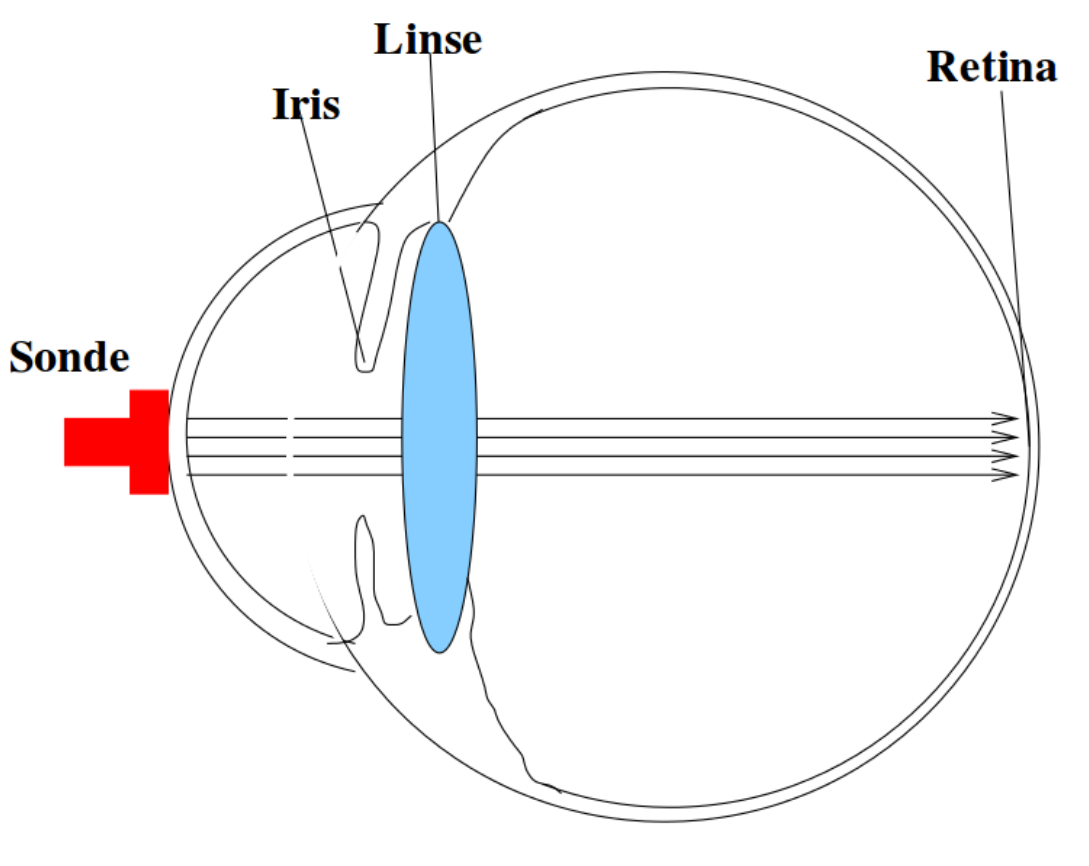
\includegraphics[height=4cm]{ressources/eyeoftheebberg.png}
  \caption{Darstellung des verwendeten Augenmodells. \cite{skript}}
  \label{abb:3}
\end{figure}
